%!TEX program=xelatex
\documentclass[14pt,a4paper]{article}

\usepackage[UTF8]{ctex}
\usepackage[T1]{fontenc}
\usepackage{textcomp}
\usepackage{mathrsfs}
\usepackage{enumerate}
\usepackage{amsmath, amssymb, amsthm}
% Hyperlinks
\usepackage{hyperref}
\hypersetup{colorlinks=true,
			linkcolor=blue,
			anchorcolor=blue,
			citecolor=cyan}
% figure support
\usepackage{float}
\usepackage{import}
\usepackage{xifthen}
\usepackage{pdfpages}

% Theorem-like statements
% Theorem
\theoremstyle{plain}
\newtheorem{thm}{Theorem}[section]
\newtheorem*{nnt}{Theorem}
% Definition
\theoremstyle{definition}
\newtheorem*{dfn}{Definition}
% Remark
\theoremstyle{remark}
\newtheorem{rmk}{Remark}[section]
\newtheorem*{nnr}{Remark}
% Lemma
\theoremstyle{plain}
\newtheorem{lem}[thm]{Lemma}
\newtheorem*{nnl}{Lemma}
% Corollary
\theoremstyle{plain}
\newtheorem{cor}[thm]{Corollary}
\newtheorem*{nnc}{Corollary}
% Axiom
\theoremstyle{definition}
\newtheorem{axm}{Axiom}[section]
\newtheorem*{nna}{Axiom}

% Title
\title{AUTO3002B Lecture Notes}
\author{H. L.}
\date{March 2020}

\begin{document}
	\maketitle
	\newpage
	\tableofcontents %Contents
	\newpage
		
	\section{控制系统设计流程}%
	\label{sec:控制系统设计流程} 
	
		\subsection{从开环到闭环}%
		\label{sub:从开环到闭环}
		
			\paragraph{Open Loop Controller}%
			\label{par:open_loop_controller}
				\ 	
				\begin{itemize}
					\item High feedback gain 
					\item Plant Model 
				\end{itemize} 

			\paragraph{Close Loop Controller}%
			\label{par:close_loop_controller}
			
				\begin{itemize}
					\item Feedback gain 
					\item Feedback
				\end{itemize} 

		\subsection{设计流程}%
		\label{sub:设计流程}
		
			\begin{enumerate}
				\item 需求分析
				\item 方案设计
				\item 采购、设计安装、集成
				\item 数学建模(简化和处理)
				\item 控制器设计
				\item 系统调试
				\item 系统测试
			\end{enumerate} 

			\subsubsection{需求分析}%
			\label{ssub:需求分析}
				
				\paragraph{功能分析}%
				\label{par:功能分析}
				
					\ 
					\begin{itemize}
						\item 控制什么
						\item 怎么控制(工作方式)
					\end{itemize} 

				\paragraph{指标分析}%
				\label{par:指标分析}
				
					\ 
					\begin{itemize}
						\item 带宽
						\item 阶跃响应 
						\item 精度(位置、速率、加速度\ldots) 
						\item \ldots
					\end{itemize}
		
				\paragraph{工作条件}%
				\label{par:工作条件}
					\ 
					\begin{itemize}
						\item 环境(外部扰动)
						\item 工况(负载变化)
						\item 约束与限制(空间、功率等)
					\end{itemize} 

			\subsubsection{方案设计}%
			\label{ssub:方案设计} 
				\begin{itemize}
					\item 结构
					\item 驱动
					\item 控制
					\item 测量
					\item 考虑因素:
						\begin{itemize}
							\item[$\triangleright$] 指标
							\item[$\triangleright$] 成本 
							\item[$\triangleright$] 可靠性 
							\item[$\triangleright$] 维护性
							\item[$\triangleright$] 安全性
							\item[$\triangleright$] 电磁兼容性 
							\item[$\triangleright$] 环境
							\ldots
						\end{itemize}  
				\end{itemize}  

			\subsubsection{采购设计安装集成}%
			\label{ssub:采购设计安装集成}
				
			\subsubsection{数学建模(及简化与处理)}%
			\label{ssub:数学建模_及简化与处理_}
		
				\begin{enumerate}
					\item 机理模型推导(理论分析和实验建模) 
					\item 模型验证与参数辨识 
				\end{enumerate} 
			
			\subsubsection{控制器设计}%
			\label{ssub:控制器设计}
		
				\paragraph{控制理论}%
				\label{par:控制理论}
				
					\begin{itemize}
						\item 古典控制
						\item 鲁棒控制
						\item 最优控制
						\item 智能控制
						\item 自适应控制
						\item 滑模控制
						\item 智能控制(模糊、神经网络)
						\item 预测控制
					\end{itemize}
			
				\paragraph{常用控制器设计方法}%
				\label{par:常用控制器设计方法}
				
				\begin{itemize}
					\item $H_\infty$ 混合灵敏度设计方法, 鲁棒性较强。 
					\item 自适应控制
					\item 多控制切换 
					\item 干扰观测器 
					\item 顺馈与前置滤波 
					\item Cascade Control Structure 
				\end{itemize}
			\subsubsection{系统调试}%
			\label{ssub:系统调试}
			
				
			\subsubsection{系统测试}%
			\label{ssub:系统测试}
			
		
	\newpage
	\section{输入信号与跟踪误差}%
	\label{sec:输入信号与跟踪误差}

		\subsection{输入信号分析}%
		\label{sub:输入信号分析}

			\subsubsection*{频谱分析}%
			
			\begin{itemize}
				\item 分析典型输入信号的幅值、变化率、二阶及高阶导数 
				\item 确定信号频带
				\item 确定元件参数、计算跟踪误差,进行控制设计
			\end{itemize}
		
		\subsection{误差系数}%
		\label{sub:误差系数}

			本课程讨论稳态误差。
			\paragraph{误差概念}%
			\label{par:误差概念}
			
			\begin{itemize}
				\item 误差 vs 偏差
				\item 稳态误差 vs 稳态偏差
			\end{itemize}

			\paragraph{静态误差系数}%
			\label{par:静态误差系数}
			\begin{itemize}
				\item 型别、$K_p$, $K_v$, $K_a$. 
				\item 适用条件:
					\begin{itemize}
						\item[$\triangleright$] 系统稳定
						\item[$\triangleright$] 输入必须是3种典型信号(阶跃、斜坡、加速度)的线性组合
					\end{itemize}  
				\item 减小静态误差的方法:
					\begin{itemize}
						\item[$\triangleright$] 提高增益 
						\item[$\triangleright$] 提高型别 
					\end{itemize}  
			\end{itemize}

			\begin{itemize}
				\item 滞后环节可减少静态误差
				\item 滞后环节应用注意事项:
					\begin{itemize}
						\item 多个中心频率不同的小幅值滞后环节比一个大幅值的好,但各环节中心频率要错开。
						\item 滞后环节要应用于低频,远离剪切频率。
						\item 滞后环节使得误差收敛速度变慢。
					\end{itemize}
			\end{itemize}


			\paragraph{动态误差系数}%
			\label{par:动态误差系数} 
			 
				\begin{itemize}
					\item $\varPhi_e(s)=\dfrac{E(s)}{R(s)} = \dfrac{1}{1+GH}$. 
					\item $t \to \infty \quad \Longleftrightarrow \quad s\to 0$. 
					\item 将$\varPhi_e$ 在$s=0$邻域内Taylor展开得
						\[
							\varPhi_e(s) = C_0+C_1s+\dfrac{C_2}{2!}s^2 + \cdots = \sum_{n=0}^{\infty} \dfrac{C_n}{n!}s^{n}
						,\]
						即
						\[
							\lim_{t \to \infty} e(t) = C_0 r(t) + C_1 \dfrac{\mathrm d r(t)}{\mathrm dt} + \dfrac{C_2}{2\ !} \dfrac{\mathrm d^2 r(t)}{\mathrm dt^2} + \cdots 
						\]
					\item 动态误差系数
						\[
							C_n = \dfrac{\mathrm d^n}{\mathrm ds^n} \left[ \dfrac{1}{1+G(s)H(s)} \right]_{s=0}
						.\] 
				\end{itemize}  
	
		\subsection{跟踪误差计算}%
		\label{sub:跟踪误差计算}

			\subsubsection{卷积法}%
			\label{ssub:卷积法}
		
				\begin{itemize}
					\item 设系统的冲激响应(或脉冲响应)为$h(t)$($h(k)$)
					\item 系统在输入$u(t)$ 下,其输出
						\[
							y(t) = h(t) * u(t) = \int_{-\infty}^\infty h(t-\tau) u(\tau) \ \mathrm d\tau 
						\]
					\item 离散情况:
						\[
							y(k) = \sum_{n=-\infty}^{\infty} h(k-n) u(n)
						\] 
					\item 实际应用中的有限卷积和
						\[
							y(k) = \sum_{n=k-N}^{k} h(k-n) u(n)
						.\]	
				\end{itemize} 

			\subsubsection{动态误差系数法}%
			\label{ssub:动态误差系数法}
			
				\begin{itemize}
					\item 用有限项逼近,一般来说取$C_0$、$C_1$、$C_2$就够了。
						\[
							\lim_{t \to \infty} e(t) = C_0 r + C_1 \dot r + \dfrac{C_2}{2!} \ddot r + \cdots 
						\]
				\end{itemize}  	
			
	\newpage
	\section{噪声}%
	\label{sec:噪声}
	
		\subsection{随机过程}%
		\label{sub:随机过程}
		
		\begin{itemize}
			\item 协方差矩阵$R$:
				\[
					\begin{split}
						r_{ij} &= \mathop{\text{cov}} \left( X_{i}, X_{j} \right) = E \left[ (x_{i}-m_{i})(x_{j}-m_{j}) \right] \\ 
							   &= \int_{-\infty}^\infty \int_{-\infty}^\infty (x_{i}-m_{i})(x_{j}-m_{j}) p(x_{i},x_{j}) \ \mathrm dx_{i} \mathrm d x_{j}\ , \quad i,j=1,\ldots ,k
					\end{split}	
				\] 
			\item 平稳随机过程:统计特性不随时间变化 \\
				期望
				\[
					m(t) = \mu
				,\]
				协方差
				\[
					r(t_1,t_2) = r(\tau)\ , \quad \tau = t_1-t_2
				.\] 
			\item 遍历性(各态历经性,ergodicity)
				\begin{itemize}
					\item[$\triangleright$]  $\implies$ ``统计平均$\Longleftrightarrow$时间平均''
					\item[$\triangleright$]  $\implies$ 随机过程平稳 
					\item[$\triangleright$]  $\not\Longleftarrow$ 平稳随机过程 
				\end{itemize}  
			\item 相关函数
				\[
					R(\tau) \triangleq E X(t) X(t+\tau) = \int_{-\infty}^\infty \int_{-\infty}^\infty x_1 x_2 p(x_1,x_2;\tau) \ \mathrm dx_1 \mathrm dx_2
				\]
				离散形式
				\[
					R(n) = \dfrac{1}{M-n} \sum_{l=0}^{M-n-1} x(l) x(l+n)
				.\] 
		\end{itemize} 
	
		\subsection{谱密度}%
		\label{sub:谱密度}
		
			\begin{itemize}
				\item 谱密度函数:平均功率密度函数
					\[
						\varPhi(\omega ) \triangleq \lim_{T \to \infty} \dfrac{1}{2T} \left| X_T (\mathrm{j} \omega ) \right|^2
					\]
					其中
					\[
						x_T (t) = \begin{cases}
							x(t), \quad -T\le t\le T\\
							0, \quad t<-T, t>T
						\end{cases} 
					\] 
					\[
						X_T(\mathrm{j} \omega ) \triangleq \mathscr F \left[ x_T(t) \right] 
					.\]
				\item 相关函数法求取:
					\[
						\varPhi(\omega ) = \int_{-\infty}^\infty R(\tau) e^{-\mathrm{j} \omega\tau}	\ \mathrm d\tau
					.\] 
			\end{itemize}  
	
		\subsection{均方误差}%
		\label{sub:均方误差}
		
			\begin{itemize}
				\item 对于线性系统,输入的功率谱密度$\varPhi_r(\omega )$ 通过$\left| G(\mathrm{j} \omega ) \right|^2$传递到输出:
					\[
						\varPhi_x(\omega ) = \left| G(\mathrm{j} \omega ) \right|^2 \varPhi_r(\omega )
					.\] 
				\item 噪声作用下,线性系统的误差(偏差)也是随机信号,噪声引起的均方误差
					\[
					\begin{split}
						\overline{e^2} &= \lim_{T \to \infty} \dfrac{1}{2T} \int_{-T}^T e^2(t)\ \mathrm dt = R_e(0) \\
									   &= \int_{-\infty}^\infty \varPhi_e(\omega ) \ \mathrm d\omega \\
									   &= \int_{-\infty}^\infty \left| G_{en}(\mathrm{j} \omega ) \right|^2 \varPhi_{n}(\omega ) \ \mathrm d\omega 
					\end{split}
					\]
					其中,$G_{en}$ 为噪声 -- 误差传递函数. 
				\item 扰动作用下线性系统的均方误差同理可求。进一步,若扰动、噪声独立,则线性系统总均方误差为二者叠加。
			\end{itemize}  

		\subsection{等效噪声带宽}%
		\label{sub:等效噪声带宽}
		
			\begin{itemize}
				\item 一个理想滤波器的带宽。使得在白噪声作用下,系统的均方输出与该理想滤波器的均方输出相等。
				\item 等效噪声带宽表征了:白噪声作用下该系统的噪声输出(误差)大小。
				\item 理想滤波器输出信号的均方输出
					\[
					\overline{x^2} = 2K_N^2 \omega_{b}
					.\] 
				\item 一般系统的均方输出
					\[
						\overline{x^2} = 2K^2_N \pi \dfrac{1}{2\pi} \int_{-\infty}^\infty \left| G(\mathrm{j} \omega ) \right|^2 \ \mathrm d\omega 
					\] 
					令
					 \[
						I\triangleq  \dfrac{1}{2\pi} \int_{-\infty}^\infty \left| G(\mathrm{j} \omega ) \right|^2 \ \mathrm d\omega 
					\]
					则一般系统的等效噪声带宽为$\pi I$ : 
					 \[
						 \overline{x^2} = 2K_N^2(\pi I)
					,\] 
					其中典型系统的$I$ 值可查表获得. 
			\end{itemize}  	


	\newpage
	\section{控制系统的设计约束}%
	\label{sec:控制系统的设计约束}
	
		\subsection{灵敏度}%
		\label{sub:灵敏度}
		
			\begin{dfn}[sensitivity]  
			\label{dfn:sensitivity}
				闭环系统传递函数的变化率与被控对象传递函数的变化率之比. 设闭环传函为$T$ ,所研究的对象(不一定是被控对象)的传递函数为$G$, 
				则灵敏度函数
				\[
					S \triangleq \dfrac{\Delta T(s) / T(s)}{\Delta G(s) / G(s)} =\dfrac{\mathrm d T}{\mathrm d G} \cdot \dfrac{G}{T} = \dfrac{\mathrm d \ln T(s)}{\mathrm d \ln G(s)} 
				.\] 
			\end{dfn} 

			\begin{rmk}[一般负反馈系统的灵敏度]  
			\label{rmk:一般负反馈系统的灵敏度}
				设系统中控制器为$K$ ,对象为$G$ ,反馈为$H$ ,系统闭环传递函数为$T$ ,一般非单位反馈闭环系统被控对象$G$ 的灵敏度为
				\[
				S^{T}_G = \dfrac{1}{1+HGK}
				.\] 
				对反馈环节变化的灵敏度为
				\[
				S^{T}_H = - \dfrac{HGK}{1+HGK}	
				.\] 
			\end{rmk} 


			\subsubsection{灵敏度函数特征}%
			\label{ssub:灵敏度函数特征}
			
				\begin{enumerate}
					\item 灵敏度表征了闭环系统对被控对象变化(模型摄动)的鲁棒性
					\item Nyquist图中,$KG$ 距离$\left( -1,\ \mathrm{j} 0 \right)$ 点的最小距离$\rho$与灵敏度函数的最大值互为倒数:
						\[
						S_{\text{max}} = \mathop{\text{max}} \left| \dfrac{1}{1+KG} \right| = \dfrac{1}{\rho}
						\]
						\[
						\rho = \mathop{\text{min}} \left| 1+KG \right| 
						.\]
					\item 相位裕度$\gamma $ 与灵敏度的关系:
						\[
						S_\textnormal{max} \ge \dfrac{1}{2\left| \sin \dfrac{\gamma}{2} \right| }
						.\]
						相位裕度给出$\rho$ 的上限,但不能给出代表鲁棒性的$S_\textnormal{max}$ 的真实值。灵敏度的最大值$S_\textnormal{max}$ 才真正反映系统的稳定程度,才是真正意义上的稳定裕度。
					\item 灵敏度函数等于扰动传递函数 --- 灵敏度反映系统对输出端扰动$d$ 的抑制特性. 
					\item 灵敏度等于误差传递函数 --- 反映系统跟踪输入信号的性能. 
				\end{enumerate} 

				综上,一般以灵敏度函数来表征\emph{反馈系统的性能},设计时要尽量压低其灵敏度。 

		\subsection{Bode积分约束}%
		\label{sub:bode积分约束}

			灵敏度函数并不能任意设计,其受到Bode积分定理的约束。

			\begin{thm}[Bode's Sensitivity Integral]  
			\label{the:bode_s_sensitivity_integral} 

			设\textbf{开环传递函数}$L(s)$ 有不稳定极点$p_1,\ldots ,p_{l}$ ,并设闭环系统\textbf{稳定} ,则系统灵敏度函数满足下列关系
				\[
					\int_{0}^{\infty} \ln |S(\mathrm{j} \omega)| \mathrm d \omega=\int_{0}^{\infty} \ln \left|\frac{1}{1+L(j \omega)}\right| \mathrm d \omega=\pi \sum_{k=1}^l \operatorname{Re}\left(p_{k}\right)-\frac{\pi}{2} \lim _{s \rightarrow \infty} s L(s)
				\]

				注意到,若设开环传递函数的相对阶 $\nu = n-m>1$ ,且开环传函稳定,则
				\[
					\int_{0}^\infty \ln \left| S(\mathrm{j} \omega ) \right| \mathrm d \omega = 0,\quad \nu>1
				.\] 
			\end{thm} 
		
			\begin{rmk}  
				由于灵敏度函数的频率积分为定值,即在Bode图上的面积是固定的,故灵敏度函数在整个频段上不能任意设计。若处理不当,则可能导致$S_\textnormal{max}$ 过大。
			\end{rmk} 

			\begin{rmk}  
				Bode积分约束只适用于\textbf{线性系统},非线性系统不受Bode积分的约束。
			\end{rmk} 

			\begin{figure}[H]
				\centering
				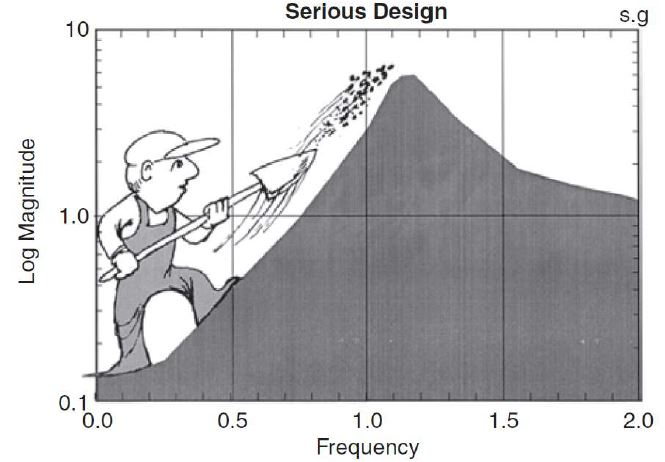
\includegraphics[width=0.9\textwidth]{./figures/bode.jpg} 
				\caption{Bode积分约束原理图示}
				\label{fig:bode}
			\end{figure} 


		\subsection{不确定性}%
		\label{sub:不确定性}
	
			\begin{itemize}
				\item 参数不确定性
				\item 未建模动态
			\end{itemize} 

			\subsubsection{不确定性的频域表示法}%
			\label{ssub:不确定性的频域表示法}
			
				\subsubsection*{(1) 加性不确定性}%
					\[
						G(\mathrm{j} \omega ) = G_0(\mathrm{j} \omega ) + \Delta G(\mathrm{j} \omega )
					,\] 
					\[
						\left| \Delta G(\mathrm{j} \omega ) \right| < l_{a}(\omega )
					.\] 
					
				\subsubsection*{(2) 乘性不确定性}%
					\[
						G(\mathrm{j} \omega ) =\left[ 1+L(\mathrm{j} \omega ) \right]  G_0(\mathrm{j} \omega ) 
					,\] 
					\[
						\left| L(\mathrm{j} \omega ) \right| < l_{m}(\omega )
					.\] 
	
				\begin{itemize}
					\item 显然,加、乘性不确定性可相互转换。
				\end{itemize}  

		\subsection{鲁棒稳定性}%
		\label{sub:鲁棒稳定性}

			\begin{dfn}[鲁棒稳定性]  
			\label{dfn:鲁棒稳定性}
				对象摄动后系统仍是稳定的。
			\end{dfn} 
		
			\paragraph{鲁棒稳定性条件}%
			\label{par:鲁棒稳定性条件}
			
				\begin{itemize}
					\item 乘性不确定性下:
						\[
							\left| \dfrac{G_0 K}{1+G_0 K} \right| < \dfrac{1}{l_{m}}
						\] 
						或
						\[
							\left| T_0(\mathrm{j} \omega ) \right| < \dfrac{1}{l_{m}(\omega )}
						.\] 
					\item 加性不确定性下:
						\[
							\left| \dfrac{K}{1+G_0 K} \right| < \dfrac{1}{l_{a}}
						\] 
				\end{itemize}  
			
				\begin{rmk}  
				当$l_{m}(\omega )\gg 1$时,$|G_0K|$很小,此时
				\[
					\dfrac{G_0K}{1+G_0K} \approx G_0 K
				,\] 
				故鲁棒稳定条件可近似化为
				\[
					\left| G_0 K \right| < \dfrac{1}{l_{m}(\omega )} \ ,\quad \forall \omega 
				.\] 

				此时就可在开环Bode图上同时标识设计性能界函数(低频)与鲁棒稳定性约束,更加清晰明了。
				\end{rmk} 

				\begin{rmk}[鲁棒稳定性条件的充分不必要性]  
				\label{rmk:鲁棒稳定性条件的充分不必要性}
				上述鲁棒稳定性条件是\textbf{充分不必要}的。从上述推导中可看出,鲁棒稳定性条件必是充分的。由于推导过程中存在三角不等式放缩,故无法得出其必要性。即:\emph{满足鲁棒稳定性条件的系统必然是鲁棒稳定的,而不满足该条件的系统是不一定鲁棒稳定的(可能鲁棒稳定)}。
				\end{rmk} 

		\subsection{带宽设计约束}%
		\label{sub:带宽设计约束}
	
			\begin{itemize}
				\item 闭环幅频特性:$3$ dB,$\omega_{b}$. 
				\item 开环频率特性:剪切频率$\omega_{c}$ ,同一数量级,关系一般有$\omega_c < \omega_{b} < 2\omega_{c}$.
				\item 相角首次滞后达到$-90^\circ $ 的频率$\omega_{p}$. 
				\item 双十频响:给定频段内,幅值误差不超过$10\%$,相位误差不超过 $10^\circ $. 
					\[
					\omega_{A 10} = \mathop{\text{min}} \left\{ \omega_{A 1.1}, \omega_{A 0.9}, \omega_{p 10} \right\} 
					.\] 
					\begin{itemize}
						\item[$\triangleright$] 双五、双三\ldots 
					\end{itemize}  
			\end{itemize}  
		
			\paragraph{响应特性}%
			
				反映系统对输入信号的响应能力,可用输入输出传递函数表征。

			\paragraph{反馈特性}%

				由反馈校正引入的特性,反映了系统稳定性、干扰抑制、指令跟踪、不确定性灵敏度等诸多性质。 

			\paragraph{带宽设计原则}%
			\label{par:带宽设计原则}
			
				\begin{itemize}
					\item 开环幅频特性低频段要大于最小性能边界,以保证信号跟随能力;
					\item 开环幅频特性要在不确定性界函数超过1之前穿过$0$ dB线,以满足鲁棒稳定性约束。
				\end{itemize}  

			\subsubsection{机械谐振}%
			\label{ssub:机械谐振}
			
			\begin{itemize}
				\item 扭转机械结构
					\[
					J \dfrac{\text{d}^2 \theta}{\text{d} t^2} + B \dfrac{\text{d} \theta}{\text{d} t} + K \theta = 0
					,\]
					固有频率
					\[
					\omega_{m} = \sqrt{\dfrac{K}{J}} 
					.\]
				\item 自由转子系统方程
					\[
					\begin{cases}
						\begin{aligned}
							J_1 \ddot \theta_1 + B \left( \dot \theta_1 - \dot \theta_2 \right) + K\left( \theta_1 -\theta_2 \right) &= T \\
							J_2 \ddot \theta_2 + B \left( \dot \theta_2 - \dot \theta_1 \right) + K\left( \theta_2 -\theta_1 \right) &= 0 \\
						\end{aligned}  
					\end{cases}
					\] 
				\item 一般设计要求
					\[
					\omega_{m} > 5 \omega_{b}
					.\] 
				\item 谐振抑制:带阻滤波器 
			\end{itemize}  

		\subsubsection{带宽设计}%
		\label{ssub:带宽设计}

			\begin{itemize}
				\item 串联校正修正剪切频率
					\begin{itemize}
						\item[$\triangleright$] 超前
						\item[$\triangleright$] 滞后 
					\end{itemize} 
				\item 反馈环节降低剪切频率
				\item 前馈、前置滤波器改善响应特性
			\end{itemize}  
			

	\newpage
	\section{Anti-Windup设计}%
	\label{sec:anti_windup设计}
	
		\begin{itemize}
			\item 执行器饱和,反馈回路失效,系统相当于进入开环状态,控制器输出不断变大. 
		\end{itemize}  	

		\subsection{积分器的Windup问题}%
		\label{sub:积分器的windup问题}
		
			\begin{dfn}[Windup]  
			\label{dfn:windup}
				积分器的累计值过大,导致执行器退出饱和时间边长,且控制器输出$\hat{u}$ 回到饱和边界之内(线性范围内)后,这一积分值作为初始条件,回导致很大的暂态响应,该现象称为Windup. 
			\end{dfn} 

		\subsection{Anti-Windup设计}%
		\label{sub:anti_windup设计}
		
			\paragraph{设计策略}%
			\label{par:设计策略}
			
				\begin{enumerate}
					\item 控制器动态由对象的实际输入信号(执行器的实际输出)驱动(即误差直接驱动比例环节,停止积分);
					\item 由对象的实际输入信号驱动时,控制器动态是稳定的。
				\end{enumerate} 

			\paragraph{基本结构}%
			\label{par:基本结构}
			
				\begin{itemize}
					\item 设控制器为双正则(相对阶$\nu=0$)最小相位系统,则可将其分解为比例项和严格正则项:
						\[
							C(s) = c_\infty + \overline{C}(s)
						.\] 
				\end{itemize}

				\begin{figure}[H]
					\centering
					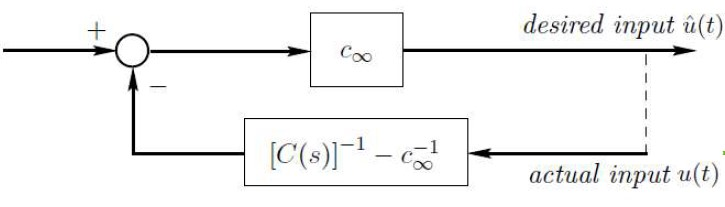
\includegraphics[width=\textwidth]{./figures/anti-windup.jpg} 
					\caption{双正则系统Anti-Windup设计}
					\label{fig:anti-windup}
				\end{figure}

		\subsection{Anti-Windup多种实现形式}%
		\label{sub:anti_windup多种实现形式}
		
			\subsubsection{第一种}%
			\label{ssub:第一种}
			
				\begin{figure}[H]
					\centering
					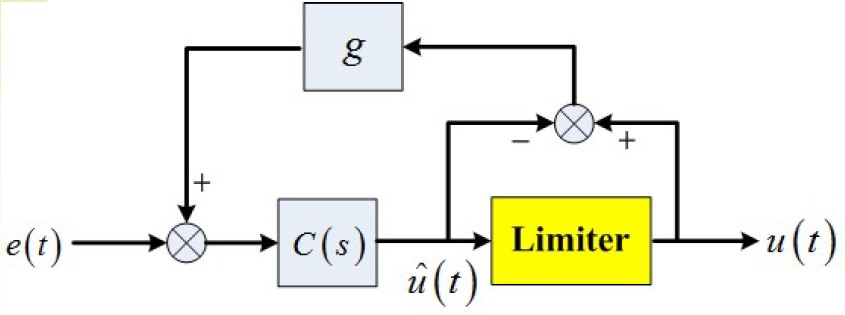
\includegraphics[width=0.9\textwidth]{./figures/aw1.jpg} 
					\caption{Anti-Windup控制器的其他形式1}
					\label{fig:aw1}
				\end{figure}
				 
				\begin{itemize}
					\item 该种实现对控制器\textbf{无}双正则、最小相位要求. 
					\item 上图中,$g$ 为静态增益 
				\end{itemize}  

			\subsubsection{第二种}%
			\label{ssub:第二种}
			
			\begin{figure}[H]
				\centering
				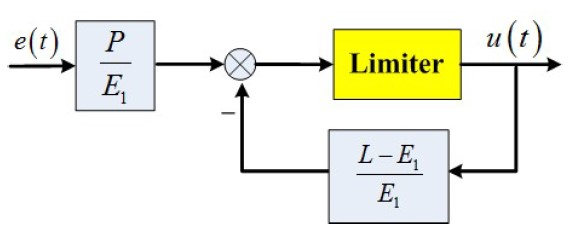
\includegraphics[width=0.9\textwidth]{./figures/aw2.jpg} 
				\caption{Anti-Windup控制器的其他形式2}
				\label{fig:aw2}
			\end{figure} 

			设控制器传递函数为
				\[
					C(s) = \dfrac{P(s)}{L(s)} 
				\]
				其中
				 \[
					L(s) = s^{n} +d_{n-1}s^{n-1} + \cdots + d_0	
				 \]
				 \[
					 P(s) = a_{m}s^{m} + a_{m-1}s^{m-1} + \cdots + a_0 \quad \left( n\ge m \right) 
				 .\] 
				 再设系统(线性工作时)闭环极点为
				 \[
				 s = -p_i \ , \quad i=1,\ldots ,N > n
				 .\] 

				\begin{itemize}
					\item 框图\ref{fig:aw2}中,$E_1(s)$ 为$n$ 阶(与分母同阶)的首一Hurwitz多项式 
						\[
							E_1 = (s+p_{k_1})\cdots (s+p_{k_n}) 
						.\] 
					\item 理论上,$E_1$ 可选为任意$n$阶首一Hurwitz多项式,只是控制性能有差异。一种经验选法:从$N$ 个闭环极点中选出最快的$n$ 个作为$E_1$ 的根。大多数情况下可获得满意的性能。
				\end{itemize} 

				\begin{rmk}  
					该种实现形式几乎无限制条件:可应用于非最小相位控制器、不稳定控制器等等. 
				\end{rmk} 


	\newpage
	\section{伺服系统}%
	\label{sec:伺服系统}

		\begin{dfn}[servomechanism]  
		\label{dfn:servomechanism}
			伺服系统又称随动系统,是用来精确地跟踪或复现某个过程的反馈控制系统。
		\end{dfn} 
	
		\subsection{伺服系统的数学模型}%
		\label{sub:伺服系统的数学模型}
		
			\begin{itemize}
				\item 伺服系统的数学模型一定有积分环节。
			\end{itemize}  

		\subsection{基本\uppercase\expandafter{\romannumeral1}型系统}%
		\label{sub:基本I型系统}
	
			\begin{itemize}
				\item 开环频率特性
					\[
						G(\mathrm{j} \omega ) = \dfrac{\omega_0}{\mathrm{j} \omega \left( \mathrm{j} \omega / \omega_1 + 1 \right)} 
					\] 
				\begin{itemize}
				\item[$\triangleright$] 以转折频率$\omega_1$为基准,取无量纲频率$\Omega = \dfrac{\omega}{\omega_1}$,得简化系统
					\[
						G(\mathrm{j} \Omega ) = \dfrac{K}{\mathrm{j} \Omega (\mathrm{j} \Omega + 1)}
					,\] 
					其中$K=\omega_0 / \omega_1$ 为无量纲增益。  
				\end{itemize} 
				\item 从性能角度考虑(相位裕度、超调、闭环幅频特性峰值),$K$ 取$1 / 2 \sim 1$ 之间数值为宜。	
				\item 基本\uppercase\expandafter{\romannumeral1}系统的等效噪声带宽
					\[
						\omega_{\text{BN}} = \pi I_2 = \frac{\omega_0 \pi}{2}
					.\]
					\begin{itemize}
						\item[$\triangleright$]	上式说明等效噪声带宽与转折频率$\omega_1$ 无关,为抑制高频噪声,一般取较小的$\omega_1$ ,令$\omega_1=\omega_0$,则$K=1$. 
					\end{itemize}  
			\end{itemize}  
		
		\subsection{改进\uppercase\expandafter{\romannumeral1}型系统}%
		\label{sub:改进I型系统}
	
		\begin{itemize}
			\item 增加一个零点(转折频率)
			\item 相当于增加一个需要设计的变量,使得两个转折频率分别决定低频增益和带宽。把带宽设计和静态增益设计分开。
		\end{itemize}  

		\paragraph{设计思路:期望频率特性法}%
		\label{par:设计思路:期望频率特性法}
		
			\begin{enumerate}[\textbf{Step} 1.]
				\item 指标确定
				\item 输入信号分析
				\item 精度分配
					\begin{itemize}
						\item 在各输入源之间分配误差,如指令输入与扰动输入。
						\item 分配方式自定,如平均分配 $e = e_r + e_d$. 
					\end{itemize} 
				\item 确定性能界函数 
				\item 跟踪误差分析 
				\item 确定低频增益
				\item 确定转折频率、剪切频率
				\item 由对象传递函数与期望频率特性得到控制器表达式
			\end{enumerate} 
	
		\begin{rmk}[正弦输入典型信号]  
		\label{rmk:正弦输入典型信号}
			有以下两个公式作为设计结论:
			\begin{itemize}
				\item 转折频率取典型工作频率
					\[
					\omega_1 = \omega_{k}
					\] 
				\item 误差幅值与增益
					\[
					e_\textnormal{max} = \dfrac{\dot \theta_\textnormal{max} }{\omega_0} \sqrt{2} 
					.\] 
			\end{itemize}  
		\end{rmk} 

		\subsection{基本\uppercase\expandafter{\romannumeral2}型系统}%
		\label{sub:基本II型系统} 

			\begin{itemize}
				\item 开环传递函数
					\[
						G(s) = K_{a} \dfrac{Ts+1}{s^2}
					\]
				\item 频率特性
					\[
						G(\mathrm{j} \Omega ) = K \dfrac{\mathrm{j} \Omega + 1}{\left( \mathrm{j} \Omega  \right)^2}
					,\]
					数字角频率
					\[
					\Omega \triangleq \omega T
					.\] 
					\begin{itemize}
						\item[$\triangleright$] 基于稳定性和噪声两方面分析,一般选取$1<K \le 2$. 
					\end{itemize}  
				\item 对数渐近幅频特性
					\[
						20\lg \left| G(\mathrm{j} \omega ) \right| = 20\left( 2\lg K_a - 2\lg \omega + \lg \dfrac{\omega}{\omega_1} \right) 
					.\]
				\item 跟踪误差
					\[
						e(t) \approx \dfrac{\ddot r}{K_a} = \dfrac{\ddot r}{\omega_1 \omega_c}  
					.\]
				\item 应用场合
					\begin{itemize}
						\item[$\triangleright$] 高精度、重载
						\item[$\triangleright$] 高性能、低带宽大型系统
					\end{itemize} 
				\item 齿隙自振荡问题:
					\begin{itemize}
						\item[$\triangleright$] 限制自振荡的幅值
						\item[$\triangleright$] 消除齿隙影响:采用两个电机拖动、采用力矩电机取消齿轮传动\ldots
					\end{itemize}  
			\end{itemize} 
			

	\newpage
	\section{调节系统}%
	\label{sec:调节系统}

		\subsection{调节系统的定义及特点}%
		\label{sub:调节系统的定义及特点}
			
		\begin{dfn}[调节系统]  
		\label{dfn:调节系统}
			调节系统是将被调量(系统的输出量)保持在设定
值上的控制系统。
		\end{dfn} 

		\subsubsection*{调节系统的特点}%
		\label{ssub:调节系统的特点}
		
		\begin{itemize}
			\item 输出量保持某个设定值
			\item 无跟踪误差要求
			\item 主要考虑\textbf{稳定性} 和\textbf{抑制扰动} 
		\end{itemize}  

		\subsection{PID控制规律}%
		\label{sub:pid控制规律}
		
			\begin{equation}
			\label{eq:pid}
			\begin{split}
				G_c(s) &= K_P + \dfrac{K_I}{s} + K_D s \\ 
					   &= K_P \left( 1+ \dfrac{1}{T_I s} + T_D s \right) 
			\end{split}
			\end{equation} 

		\subsection{调节系统的类型}%
		\label{sub:调节系统的类型}
	
		调节系统主要有两种类型
			\begin{itemize}
				\item 积分加一阶模型
					\[
						G(s) = \dfrac{K}{s(Ts+1)}
					,\] 
					或近似的,二阶惯性模型
					\[
						G(s) = \dfrac{K}{(T_1 s+ 1)(T_2 s + 1)} \ , \quad T_1 \gg T_2
					.\] 
				\item 一阶加时间滞后模型
					\[
						G(s) = \dfrac{K}{Ts+1} e^{-\tau s}
					.\] 
			\end{itemize} 

		\subsection{PID系统设计}%
		\label{sub:pid系统设计}
		
			针对积分加一阶对象,主要讨论两种控制方案
			\begin{itemize}
				\item PD控制,调节系统阻尼系数 
					\begin{itemize}
						\item[$\triangleright$] 被控对象一般为运动体,调节目的以提供阻尼为主。加上PD后整个系统的低频数学模型仍是二阶的。
					\end{itemize}  
				\item PI控制,考虑相角裕度,提高系统精度
			\end{itemize}  

			\subsubsection{PD策略}%
			\label{ssub:pd策略}
			
				\[
					G_c(s) = K_P + K_D s
				.\] 

				\begin{itemize}
					\item $K_P$ 决定系统固有频率$\omega_{n}$ ,反映响应速度;
					\item $K_D$ 决定系统阻尼系数$\zeta$. 
				\end{itemize} 
				
				\begin{rmk}[动特性]  
				\label{rmk:动特性}
					一般对于调节系统,由于期望的固有频率一般很低,远低于执行机构、功放级、测量元件等,故以上成分的动特性在系统工作频段内可忽略不计。即,PID控制器已经包含了除被控对象外所有的机构的特性。
				\end{rmk} 

			\subsubsection{PI策略}%
			\label{ssub:pi策略}
			
				\[
					G_c(s) = K_P \left( 1+ \dfrac{1}{T_{i} s} \right)	 
				.\] 

				对于要求无静差,且存在高频噪声的对象,宜采用$PI$ 控制。

				\begin{itemize}
					\item 欲取得最大相角裕度的\textbf{对称整定法} 
				\end{itemize}  

		\subsection{过程控制系统设计}%
		\label{sub:过程控制系统设计}
		
		\begin{itemize}
			\item 过程控制系统一般存在纯延迟环节
			\item 虽同样采用PID控制率,但是微分增加阻尼的效果并不明显,故P和I起主要作用. 
			\item 参数整定:临界比例度法,Ziegler--Nichols参数整定表 
			\item 参数整定原则:
				\begin{enumerate}
					\item 微分项转折频率大于带宽
					\item 积分项转折频率为剪切频率的$\dfrac{1}{2} \sim \dfrac{1}{4}$ 
					\item 比例项决定剪切频率处特性
					\item 宜采用幅值裕度衡量系统相对稳定性
				\end{enumerate} 
		\end{itemize}  


	\newpage
	\section{多回路系统}%
	\label{sec:多回路系统}

		\subsection{多回路系统设计}%
		\label{sub:多回路系统设计}
		
			\subsubsection{单回路系统的局限性}%
			\label{ssub:单回路系统的局限性}
	
				三大矛盾:
				\begin{enumerate}
					\item 系统中噪声大,输入信号的频谱不宽:要求系统的带宽要窄,但 带宽变窄,干扰抑制的效果变差;
					\item 干扰的频谱宽,干扰量大:即使做到了最大带宽,仍有可能满足不了干扰抑制的要求; 
					\item 要求系统的频率响应较宽:系统的带宽因受鲁棒稳定性约束却做不到。
				\end{enumerate} 

			\subsubsection{对回路系统设计思路}%
			\label{ssub:对回路系统设计思路}
			
			\begin{itemize}
				\item 用宽带宽的内回路抑制干扰;
				\item 用窄带宽的外回路保证精度;
				\item 内外回路频率错开
					\[
					\omega_{no} \le \dfrac{1}{5} \omega_{ni}
					\] 
				\item 先调试内回路,再调试外回路;
				\item 调试外回路时,内回路近似为比例环节。
			\end{itemize} 

		\subsection{串级调节系统}%
		\label{sub:串级调节系统}
		
			在大滞后对象中选取能够比较快反映扰动和控制作用的中间变量作为副变量。设计副回路利用副调节器镇定副变量,即可大大改善主变量的调节性能。 

			\begin{itemize}
				\item 主调节器的输出作为副调节器的设定值;
				\item 副回路响应较为迅速,负责``先调''、``粗调''、``快调'';
				\item 主回路响应较慢,负责``后调''、``细调''、``慢调'',消除副回路未能完全克服的干扰影响;
				\item 鉴于响应速度不同的特点,两个调节器的时间常数很自然地相差较大,频率自然错开。
			\end{itemize} 


		\subsection{复合控制}%
		\label{sub:复合控制}
	
			\begin{figure}[H]
				\centering
				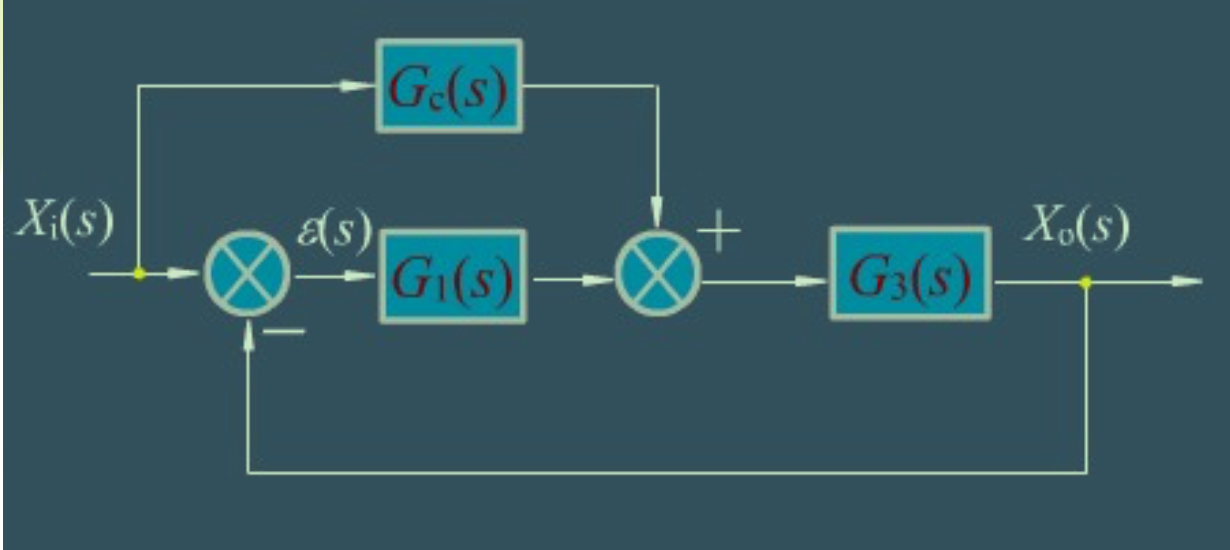
\includegraphics[width=1\textwidth]{./figures/feedforward.png} 
				\caption{复合控制系统控制框图}
				\label{fig:ff}
			\end{figure}

			\begin{itemize}
				\item 思路:顺馈补偿+反馈闭环
				\item 关于顺馈:
					\begin{itemize}
						\item[$\triangleright$] 增加顺馈补偿通道,系统稳定性不受影响(特征多项式不变);
						\item[$\triangleright$] 采用顺馈,理论上可做到消除稳态误差:
							\[
								\varPhi_e(s) = \dfrac{\varepsilon(s)}{X_{i}(s)} = \dfrac{1-G_c G_3}{1+G_1 G_3}
							\] 
							只需使得
							\[
								G_c(s) = \dfrac{1}{G_3(s)}
							.\] 
					\end{itemize}   
			\end{itemize}  


	\newpage
	\section{扰动响应及抑制}%
	\label{sec:扰动响应及抑制}

		\begin{dfn}[disturbance]  
		\label{dfn:disturbance}
			除给定值外,凡是能引起被控量发生变化的因素,都可划入扰动的范围。扰动是对系统的输出产生不利影响的信号。
		\end{dfn} 

		\begin{dfn}[noise]  
		\label{dfn:noise}
			混在有用信号上的外加信号叫噪声,一般由测量引入,难以分离。
		\end{dfn}

		\paragraph{干扰与噪声的区别}%
		\label{par:干扰与噪声的区别}
		
		\begin{itemize}
			\item 作用点:干扰一般和控制量作用点相同;噪声更多作用于测量元件上
			\item 作用机理:干扰直接作用于被控对象;噪声混入反馈信号从而间接影响被控量
			\item 特性:干扰大多可被测量与估计,频带较窄;噪声为随机信号,频谱范围宽
			\item 抑制方法:噪声一般只能通过降低带宽(等效噪声带宽)来抑制,常与系统跟踪性能矛盾。
		\end{itemize}  
	
		\subsection{扰动响应与误差分析}%
		\label{sub:扰动响应与误差分析}
			\begin{figure}[H]
				\centering
				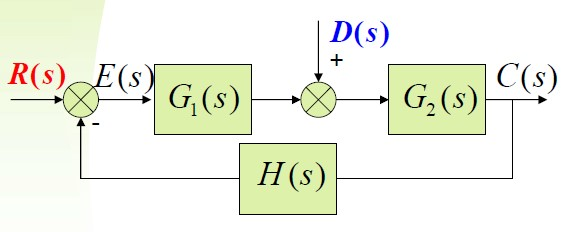
\includegraphics[width=0.8\textwidth]{./figures/disturbance.jpg} 
				\caption{研究扰动响应的系统控制框图}
				\label{fig:disturbance}
			\end{figure}

			\begin{dfn}[扰动响应]  
			\label{dfn:扰动响应}
				系统的扰动到输出的传递函数
				\[
					\varPhi_d (s) = \dfrac{C(s)}{D(s)} = \dfrac{G_2}{1+G_1 G_2 H}
				.\] 
			\end{dfn} 

			\begin{dfn}[扰动误差]  
			\label{dfn:扰动误差}
				扰动作用产生的误差为扰动误差
				\[
					e_\textit{ssd}  = \lim_{s \to 0} sE(s) = - \lim_{s \to 0} s\cdot \dfrac{G_2 H}{1+G_1 G_2 H}\cdot D 
				.\] 
			\end{dfn} 

			\paragraph{减小扰动误差的方法}%
			\label{par:减小扰动误差的方法}
			
				\begin{itemize}
					\item 增加偏差点到扰动作用点之间的放大系数或积分环节个数($G_1$) 
					\item 采用PI策略(同时引入积分环节和一个附加的零点以保证系统稳定性) 
					\item 采用顺馈或扰动观测器
				\end{itemize} 

		\subsection{扰动观测器}%
		\label{sub:扰动观测器}
		
			诚然,若扰动可测,且扰动与系统状态无关,则可以使用顺馈的方式从理论上完全消除扰动对于系统输出的影响。若扰动与系统状态有明确的函数关系,在状态可测的情况下仍可以通过辨识扰动模型的参数,从而使用顺馈进行补偿。但是,若扰动本身不可测呢?

			扰动观测器的基本思想是将\emph{外部干扰及模型参数变化}造成的\emph{实际对象与名义模型之间输出的差异}等效到控制输入端。即观测出等效干扰,在控制中引入等效补偿,实现对干扰的完全抑制。

			\begin{figure}[H]
				\centering
				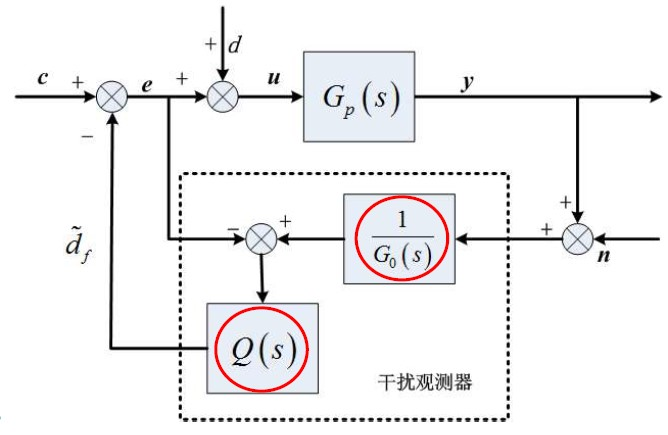
\includegraphics[width=0.8\textwidth]{./figures/disturbance_observer.jpg} 
				\caption{扰动观测器}
				\label{fig:disturbance-observer}
			\end{figure} 

			图\ref{fig:disturbance-observer}中:
			\begin{itemize}
				\item $Q$ 为一低通滤波器
				\item $G_0$ 为对象的名义模型
				\item $\tilde d_f$ 为扰动的估计值
			\end{itemize} 

			\subsubsection{低通滤波器的设计}%
			\label{ssub:低通滤波器的设计}
				
			图\ref{fig:disturbance-observer}中低通滤波器$Q(s)$ 的引入,有助于:
			\begin{itemize}
				\item 抑制模型摄动
				\item 抑制干扰
				\item 降低对噪声的敏感度
			\end{itemize} 

			\begin{rmk}[Q的带宽]  
			\label{rmk:q的带宽}
				$Q(s)$ 的带宽应覆盖扰动和输入信号的频带,且在满足抑制扰动的同时,应尽可能地窄。
			\end{rmk} 

			\paragraph{Q的设计原则}%
			\label{par:q的设计原则}
			
				\begin{itemize}
					\item 保证物理可实现性:$Q$ 的相对阶不能小于名义模型$G_0$ 的相对阶;   
					\item 鲁棒稳定性:设$G_p = G_0\left( 1+\Delta  \right) $ ,则需保证
						\[
							\|\Delta(s) Q(s)\|_{\infty} \le 1
						.\] 
				\end{itemize}  

			\paragraph{二项式滤波器}%
			\label{par:二项式滤波器}
			
				\begin{equation}
				\label{eq:LPF}
				Q(s) = \dfrac{\sum\limits_{k=0}^{N-r} \alpha_{Nk}\left(\tau s \right)^{k}}{\left( \tau s+1 \right)^{N}} 
				\end{equation} 
				其中,
				\[
				\alpha_{Nk} = \dfrac{N!}{\left( N-k \right) !} 
				,\] 
				$N$ 与$r$ 分别为$Q$ 的阶次和相对阶,$\tau$ 为滤波时间常数。

			\begin{figure}[H]
				\centering
				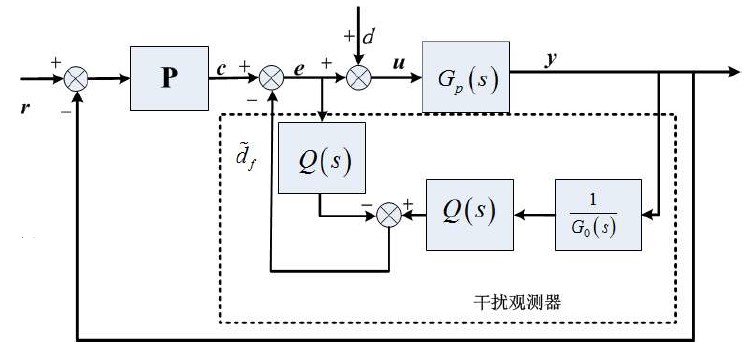
\includegraphics[width=0.8\textwidth]{./figures/do1.jpg} 
				\caption{扰动观测的实现}
				\label{fig:do}
			\end{figure}





\end{document}
